\documentclass[11pt, letterpaper]{article}
\usepackage[utf8]{inputenc}
\usepackage[letterpaper, margin=1in]{geometry}
\usepackage{amsmath}
\usepackage{amssymb}
\usepackage{amsthm}
\usepackage{graphicx}
\usepackage[font=scriptsize]{caption}
\usepackage{subcaption}
\graphicspath{ {./Report Images/} }
\captionsetup{justification=raggedright, singlelinecheck=false}
\usepackage{xcolor}
\usepackage{multicol}
\usepackage[title]{appendix}
\usepackage[left=1cm, right=2cm]{geometry}
\newgeometry{left=1.4cm,right=1.4cm,bottom=2cm, top=1cm}

\title{Project 1: Redwoods Data Report}
\author{Devin Ti and Ryan Tang}
\date{October 13th 2022}

\begin{document}
\maketitle

\section{Summary}
\subsection{Paper Overview}
The Redwoods paper provides a case study demonstrating that utilization of a sensor network could enable a more in-depth analysis of an organism. With better technology, we can capture much more data in longitude and granularity than we previously could using a single, limited piece of equipment.
The motivation comes from numerous questions and requests from the local biologists. These scientists have many intriguing things to study, but the poor data availability hinders observability and precludes
the possibility. The team decided on this study because the coastal redwood has a known micro-climate phenomenal variation within and across the days. It is the perfect subject for the demonstration and a great testbed to discover any limitations. With all these, the team showed that the newly acquired data reveals a much more complex dynamic system that Biologists have never been able to observe directly. The analysis also confirms that the redwood experiences substantial variation in temperature, moisture, and light levels throughout the day at its weather fronts.

\subsection{Data Collection}
The sensor network consists of 33 motes, a central network gateway, and an internal data logging backup. Each sensor is perfectly weathered while safely exposing the sensors. It has its battery, operating system, a top sensor for incident photosynthetically active radiation (PAR), and a bottom sensor for temperature, humidity, and reflected PAR. On average, they placed sensors across the entire redwood, mainly near the trunk and within a 1-meter radius, with 2-meter spacing. The placement started at the 15-meter mark and went up to the pinnacle of the tree 67-meter. Such placement and spacing enable the sensors to capture the microclimate of the tree with the entire spectrum rather than the broader climate, which is our point of interest. Another detail is that they placed most of their sensors on the west side of the tree because it has a ticker canopy to shield it against environmental effects.

After nailing down the deployment plan, we have a few more things to confirm. The length of deployment is 44 days, starting on Tuesday, April 27th, 2004, at 5:10 pm and ending on Thursday, June 10th, 2004, at 2:00 pm. It also has a 5-minute sampling frequency. To put it precisely, it is up 4s every 5-minute to log the current sensor values, send it out through the network, and back to sleep again --- a 1.3\% duty cycle. In case of network failure, the readings were saved in the local logging system, which was retrieved after the experiment; however, it has a limited storage space and only works when the sensor battery is still up. 

The sensor cluster has an internal data collection framework, TinyDB. All data were collected through this framework using a SQL-like language and transmitted through the network most of the time. In particular, it retrieves four pertinent readings: relative humidity, temperature, incident PAR, and reflected PAR. In addition to the fours, it also records the nodeId, the parent nodeId, query time, and epoch. These are the relevant time and height dimensions used for keying purposes. 


\section{Data Cleaning}
\subsection{Data Description}
The data comes in two separate files.
\begin{enumerate}
    \item \textit{sonoma\_log} corresponding to measurements stored in the internal logging system of each sensor.
    \item \textit{sonoma\_net} corresponding to measurements stored in a network cloud system by each sensor.
\end{enumerate}
The two datasets correspond to how the data is collected. All sensors capture measurements at a given time and attempt to write the measurements to a network database. Since the transmission might fail due to network issues, the sensor also writes the measurement to an internal database resulting in the log dataset. There are several implications of this process, and we will address them in the following sections.
\begin{enumerate}
    \item There are differences in how the various quantities are measured in the log and the network dataset. This is displayed in Figure \ref{fig1}, where histograms are plotted for the variables of interest. We have found that the differences are largely due to outliers.
    \item For a given sensor and a given time, there might be repeated measurements, one for the log and one for the sensor. In fact, we have found multiple sensors with multiple log and net readings at a given epoch. See Section 2.6 for details.
    \item Data yield is also a concern; The paper mentioned that we have around 800k data point yield, but we only have around 415k data points in the given dataset after combining both the logged and network values. The actual effective yield is much lower due to duplicate or off measurements.
\end{enumerate} \\

\begin{figure}[!h]
\centering
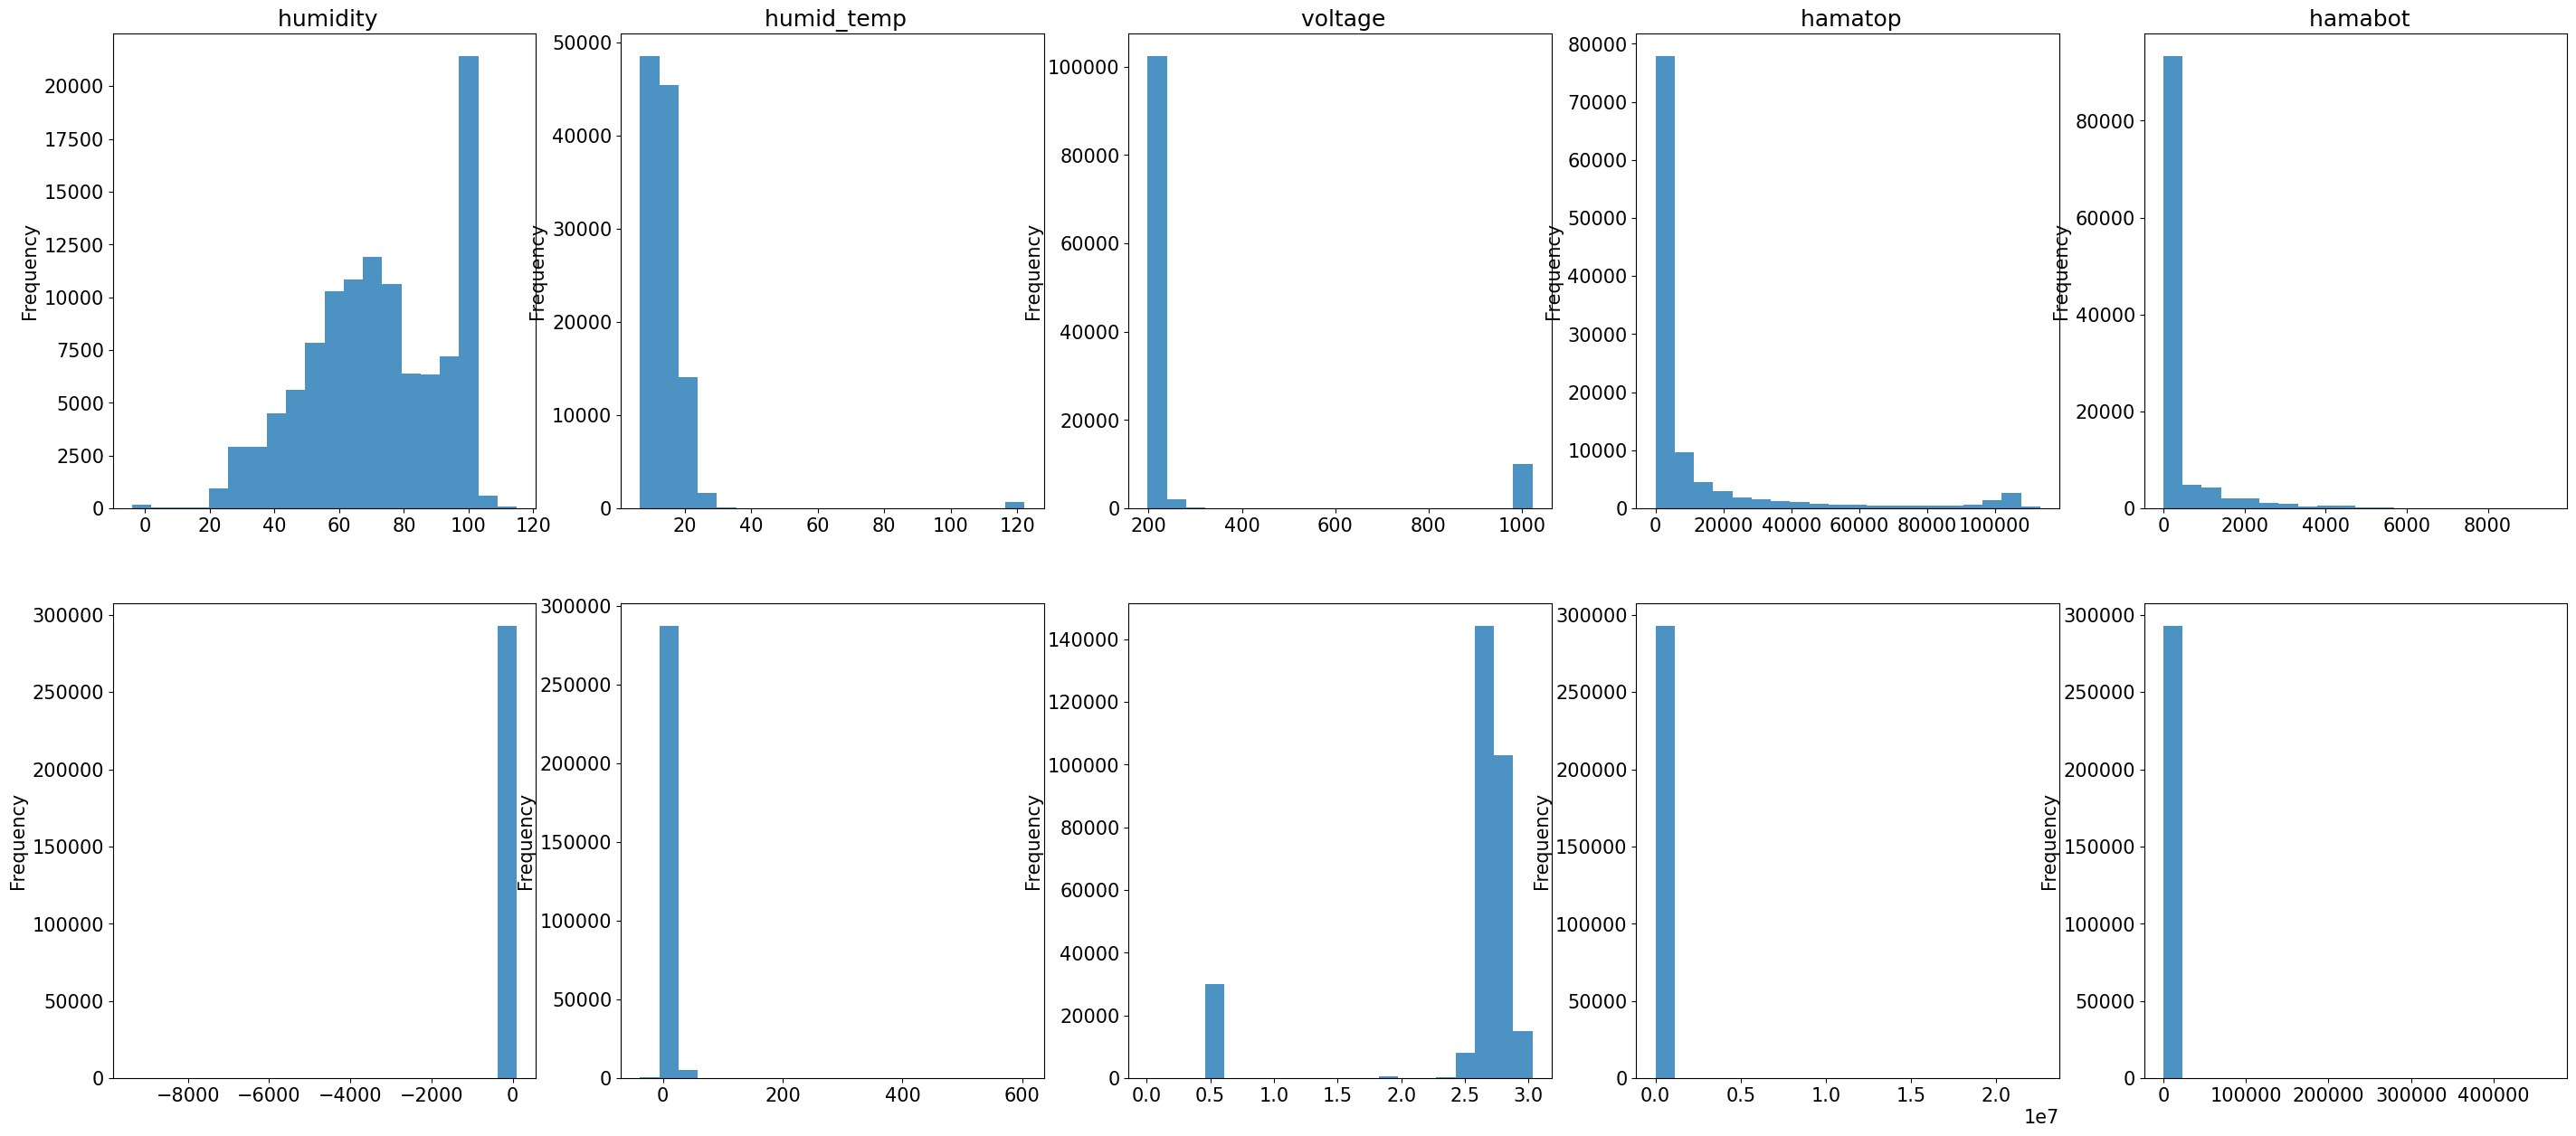
\includegraphics[width=1.0\textwidth]{Report Images/Fig1.png}
\caption{Histograms for 5 variables: humidity, temperature, voltage, incident PAR, reflected PAR. Top Row: Network data, Bottom Row: Log Data}
\label{fig1}
\end{figure}

\subsection{Part A: Histograms \& Converting Ranges}
Figure \ref{fig1} is meant to be compared to Figure 3a in the paper. This highlights two issues: 1) That the ranges of the data are not necessarily the same between the \textit{sonoma\_log} and the \textit{sonoma\_net} datasets, and 2) Some of the measurement units are different from that of the paper, as can be seen by the vastly different ranges. We see this in the PAR variables \textit{hamatop} and \textit{hamabot}. This is expressed in Tables \ref{table:sonoma_net_pre_transform} and \ref{table:sonoma_log_pre_transform}, where we plot several statistics for each variable of interest. Therefore, one should not concatenate the two files without any pre-processing.
\\ \\
We conducted two transformations for hamatop and hamabot in both datasets. We posit that the collected PAR number is under the unit of LUX, and we need to convert it down to $\mu mol/m^2/s$ by dividing it by $54$. 
\\ \\
Also, For voltage in \textit{sonoma\_net},  we note that the range is quite different from \textit{sonoma\_log} and that in the paper. However, we could not find the appropriate conversion and thus did not convert it even though it has some relevance for data cleaning afterward.
\\


Tables \ref{table:sonoma_net_post_transform} and \ref{table:sonoma_log_post_transform} show the statistics of the variables after the transformations. As we can see, the ranges of the two histograms are still not equal. This is due to outliers. We will address this in Part B.


\begin{figure}[h!]
\captionsetup{justification=centering}
\centering
\begin{tabular}{ |c|c|c|c|c|c| } 
    \hline & Median & Mean & SD & 25 Percentile & 75 Percentile \\ 
    \hline
    Humidity & 72.05 & 72.12 & 21.32 & 57.10 & 92.60 \\
    Temperature & 12.98 & 14.27 & 9.84 &	10.11  & 16.08\\
    Voltage & 223.0 & 292.79 & 227.22 & 218.0 & 227.0 \\
    Hamatop (incident PAR) & 10870.34 & 11,521.65  & 24,962.81 & 0.0 & 8,436.36 \\
    Hamabot (Reflected PAR) & 245.53 & 271.94 & 805.30  & 0.0 & 0.0 \\
    \hline
%\caption{Statistics for \textit{sonoma\_net} Pre-Transformation}
\end{tabular}
\captionof{table}{Statistics for \textit{sonoma\_net} Pre-Transformation}
\label{table:sonoma_net_pre_transform}
\end{figure}

\begin{figure}[h!]
\captionsetup{justification=centering}
\centering
\begin{tabular}{ |c|c|c|c|c|c| } 
    \hline & Median & Mean & SD & 25 Percentile & 75 Percentile \\ 
    \hline
    Humidity & 61.58 & 61.41  &	31.06 	& 40.02 	 & 80.19 \\ 
    Temperature & 14.71 & 15.02 	& 5.69 	& 10.86 	& 18.81 \\
    Voltage & 2.69 & 2.50 	& 0.64  & 2.62  & 2.77 \\
    Hamatop (incident PAR) & 0.0 & 10,870.34 & 48,422.14 & 0.0 & 6,762.33 \\
    Hamabot (Reflected PAR) & 0.0 & 245.53 & 1,180.33 & 0.0 & 0.0 \\
    \hline
\end{tabular}
%\caption{Statistics for \textit{sonoma\_log} Pre-Transformation}
\captionof{tabe}{Statistics for \textit{sonoma\_log} Pre-Transformation}
\label{table:sonoma_log_pre_transform}
\end{figure}

\begin{figure}[h!]
\captionsetup{justification=centering}
\centering
\begin{tabular}{ |c|c|c|c|c|c| } 
    \hline & Median & Mean & SD & 25 Percentile & 75 Percentile \\ 
    \hline
    Hamatop (incident PAR) & 0.0 & 213.36 & 462.27 & 0.0 & 156.22\\
    Hamabot (Reflected PAR) & 0.0 & 5.03	& 14.91 & 0.0 & 0.0 \\
    \hline
\end{tabular}
\captionof{table}{Statistics for \textit{sonoma\_net} after change of units}
\label{table:sonoma_net_post_transform}
\end{figure}

\begin{figure}[h!]
\captionsetup{justification=centering}
\centering
\begin{tabular}{ |c|c|c|c|c|c| } 
    \hline & Median & Mean & SD & 25 Percentile & 75 Percentile \\ 
    \hline
    Hamatop (incident PAR) & 0.0 & 201.30 & 896.71 & 0.00 & 125.23 \\
    Hamabot (Reflected PAR) & 0.0 & 4.55 & 21.86 &  0.00 & 0.00 \\
    \hline
\end{tabular}
%\caption{Statistics for \textit{sonoma\_log} after change of units}
\captionof{table}{Statistics for \textit{sonoma\_log} after change of units}
\label{table:sonoma_log_post_transform}
\end{figure}

\subsection{Part B: Missing Data}
There are also several sensors with missing data recorded in at least one of the 4 fields. We filter these data points out and present the statistics in Table \ref{table:data_info}. There are many lines with missing data, forming 2.746\% and 3.706\% of the log and network datasets, respectively.

\begin{figure}[h!]
\captionsetup{justification=centering}
\centering
\begin{tabular}{ |c|c|c|c|c| } 
    \hline & num Original & num After Missing Data Removed & num Missing & \% Missing \\
    \hline
    \textit{sonoma\_log} & 301,056 & 292,786 & 8,270 &2.75\\ 
    \textit{sonoma\_net}  & 114,980 & 110,718 & 4,262 & 3.71\\
    \hline
\end{tabular}
\captionof{table}{Size of log and network data sets, before and after missing data is removed.}
\label{table:data_info}
\end{figure}

\subsection{Part C: Combining Auxiliary Location Data}
The next step is combining the measurements with the sensors' spatial information. This is done by joining the mote-location dataset with sonoma-log and sonoma-net on the ID and nodeid attributes. The resulting datasets have 14 columns each. The column names are listed in Appendix A.


\subsection{Part D \& E: Outliers}
In this section, we further cleaned the data by removing outliers. We consider 2 types of outlier data measurements. 
\begin{enumerate}
    \item Outliers data measurements have abnormally high or low values of one of the variables of interest.
    \item Repeated measurements where a node has multiple measurements at a single epoch.
\end{enumerate}
Point 1. can be done in 2 ways. Firstly we combine the net and log data, threshold points are then set visually, and we classify data points beyond thresholds as outliers and remove them. To do this, we start with the histogram in Figure \ref{fig3:combined_hist}. 

\begin{figure}[h!]
\centering
\captionsetup{justification=centering}
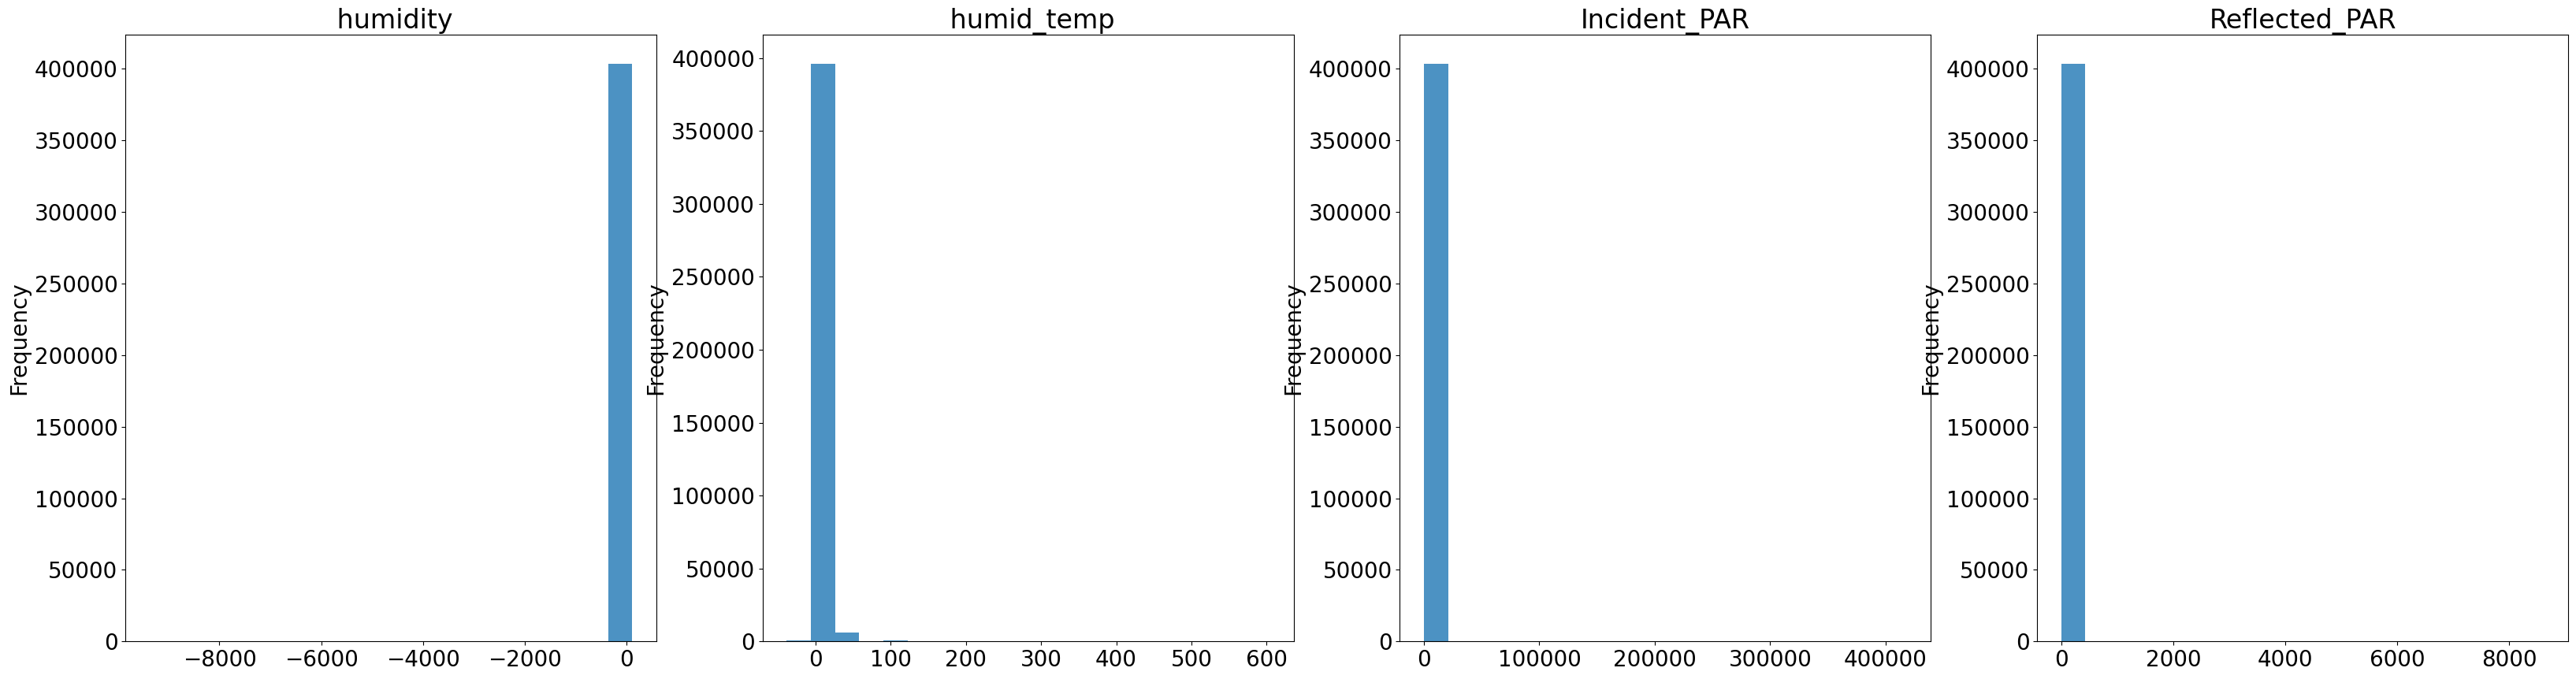
\includegraphics[width=1.0\textwidth]{Fig3_combined_hist.png}
\caption{Histograms of humidity, temperature, incident PAR and reflected PAR before the outlier removal}
\label{fig3:combined_hist}
\end{figure}

We set the following manual thresholds for the 4  variables, humidity, temperate, incident PAR, and reflected PAR.

\begin{itemize}
    \item humid: \textit{humid} $<$ 5
    \item Temperature: \textit{Temperature} $>$  80
    \item Incident\_PAR: \textit{Incident\_PAR} $>$  2100
    \item Reflected\_PAR: \textit{Reflected\_PAR} $>$  2000
\end{itemize}
In total, 1407 points hit one of the conditions, with most data points (n=874) having a negative humidity. We further found that one data point is largely responsible for the large values in incident PAR and reflected PAR. After cleaning, the resulting histograms are shown in \ref{fig3:combined_hist_after_clean}. We can see that the histograms look much better, and the distribution of each variable is much more reasonable.

\begin{figure}[h!]
\centering
\captionsetup{justification=centering}
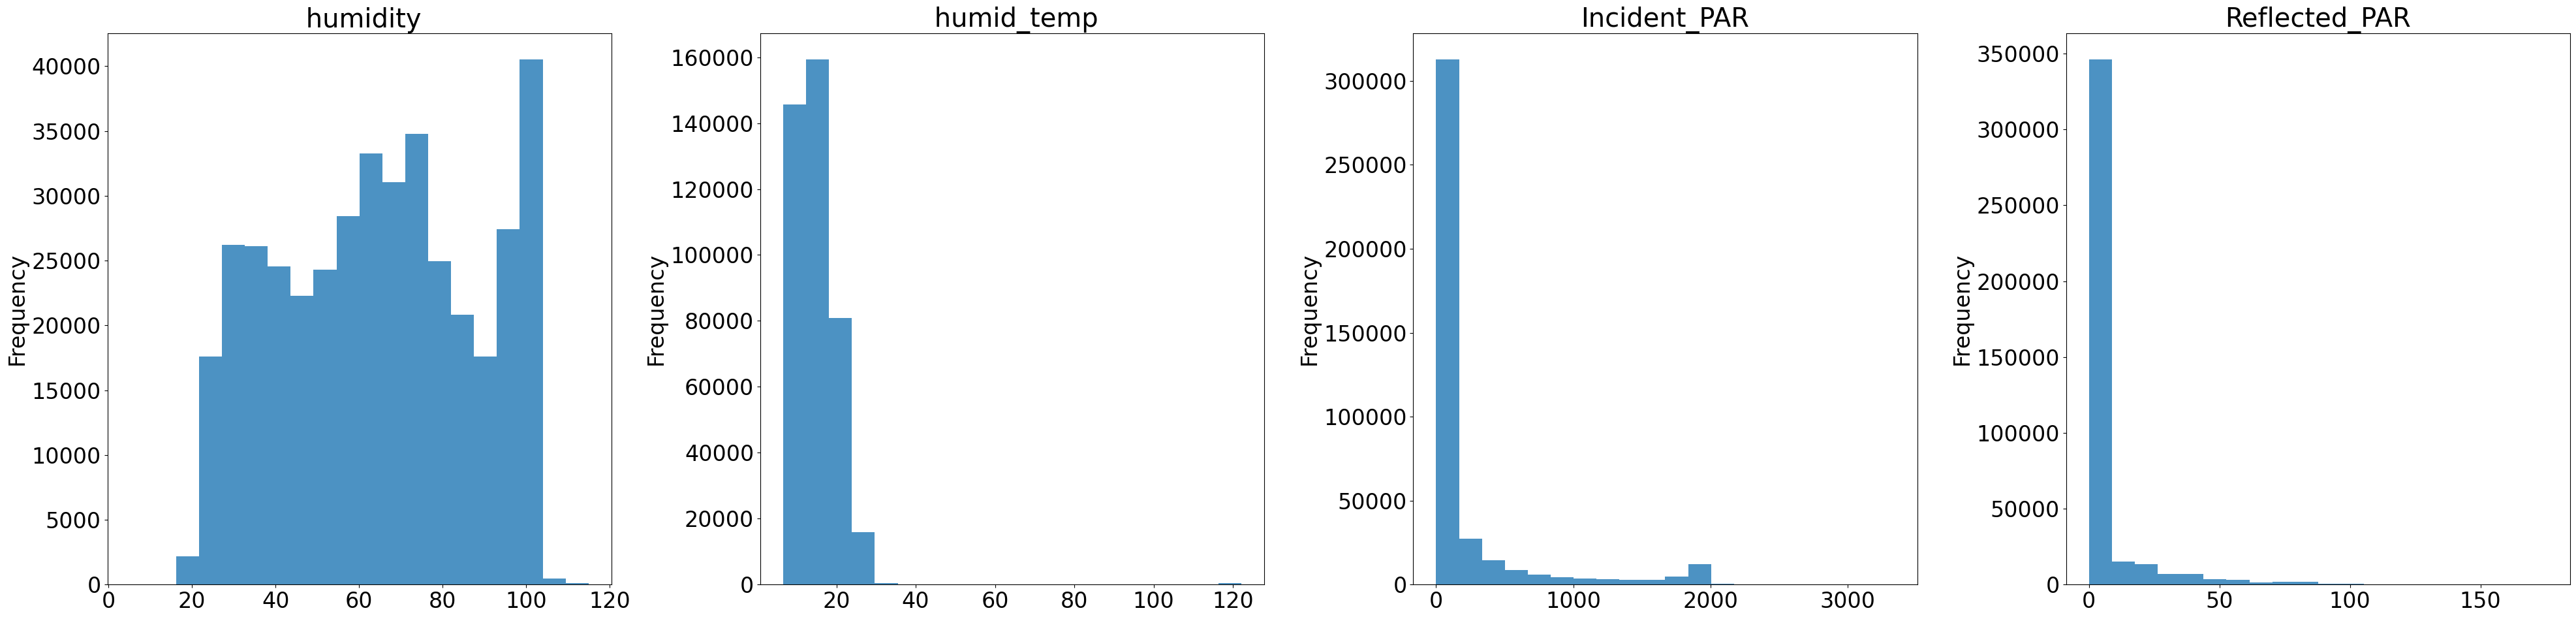
\includegraphics[width=1.0\textwidth]{Fig4_combined_hist_after.png}
\caption{Histograms of humidity, temperature, incident PAR, and reflected PAR after the outlier removal}
\label{fig3:combined_hist_after_clean}
\end{figure}


\subsection{Part E: Additional Pre-Processing}
We consider two additional cleaning measures. We are removing readings at low voltages and removing repeated readings. With all the pre-processing, we end up with a dataset of $287,207$ in size.
\\ \\
\underline{Low Voltage}: The paper mentions that all readings taken where the node's voltage was outside of the range of 2.4 and 3 were removed. This range corresponds to the operational capacity of the sensor battery. If a sensor operates under a low battery condition, the outputting measurement is unreliable; thus, we can assume that readings taken outside this range are highly erroneous. As a first check, all outliers detected in Section 3.4 have voltages below 2.4, with the highest having 2.3291 volts and the lowest ha 0.00906 volts. To keep in line with the paper, we removed an additional 28,699 data points where the voltage was outside $[2.4, 3]$. Also, note that we could only conduct this step for measurements from the log data.
\\ \\
\u,nderline{Repeated Measurements}: As mentioned in Section 2.1. There are numerous data entries where the nodeid and the measurement epoch (time of measurement) are the same. This implies multiple measurements exist for the same node at the same period. We want to remove such duplicate entries because they can potentially skew the statistics and introduce un-welcomed bias. One way this duplication occurs is when both a log and a net value get saved for a given node and epoch. In total, there are $72,755$ node-epoch pairs where this duplication occurs. After inspecting these pairs, we find that the measurements are often the same, but there can be deviations in some cases. We also found that duplication can occur because the sensor writes multiple times in a short time to the network or the log; this was the case for sensor node 118. To de-duplicate, we take a random data point with a preference for the network measurements when all the measurements are the same. We take the smaller measurements if they are different. 


\section{Exploratory Data Analysis (EDA)}
\paragraph{Correlation Analysis}
For exploration purposes, we first plot the four measurements in a pair-wise plot to see if any relationship exists. To avoid clutter and focus on the high-level correlation, we aggregated the sensor data by hour and height, assuming that the relationship predominantly occurs within a day and inter-day behaviors, more or less, follow a periodic pattern. As shown in Figure \ref{fig:pairwise}, Temperature and Humidity have a strong negative correlation. This makes sense. And both PAR measures showed a somewhat negative correlation with Humidity and a positive correlation with Temperature. This matches the intuition that we should expect low PAR during the night and early morning and high PAR during the day when the sun is out. The day is also the time that tends to have higher temperatures and lower humidity. Of course, there are exceptions, like when the redwood experience with large mist that can block the radiation.
\begin{figure*}[h!]
\centering
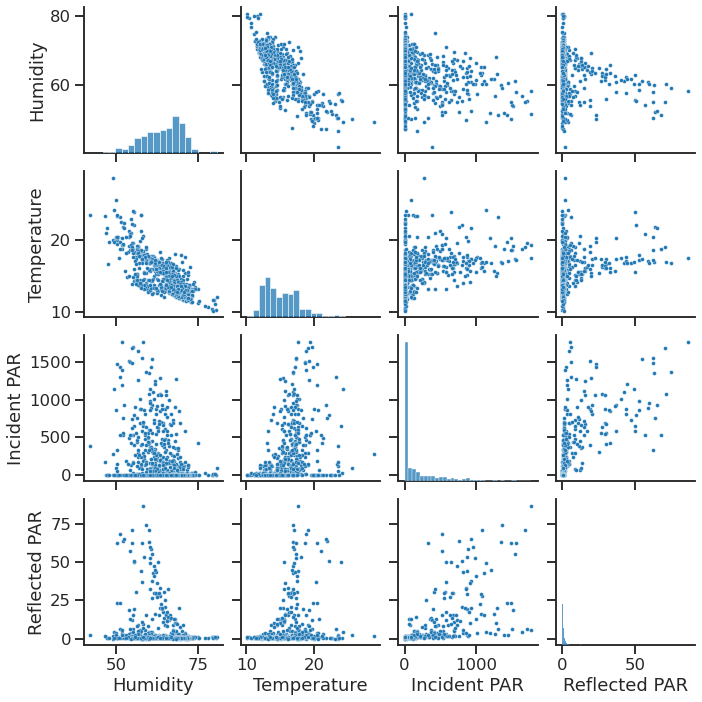
\includegraphics[width=0.65\textwidth]{eda_3.1.png}
\captionsetup{justification=centering}
\caption{Feature Pairwise Plot}
\label{fig:pairwise}
\end{figure*}


\paragraph{Intra-Day Behavior}
We can see the intra-day behavior more explicitly in the following plots (Figures \ref{fig:par-intra-day} and \ref{fig:th-intra-day}). PAR usually shoots up around 6 or 7 o'clock when the sun is up, reaches its highest around 4 PM, and shoots down after 6 PM. Temperature follows a similar pattern, with high measurements during the day and low measurements during the night, but with lower variances than PAR. On the other hand, Humidity expresses stable behavior across the day with slightly lower measurements between 10 AM to 5 PM.
\begin{figure*}[h!]
\centering
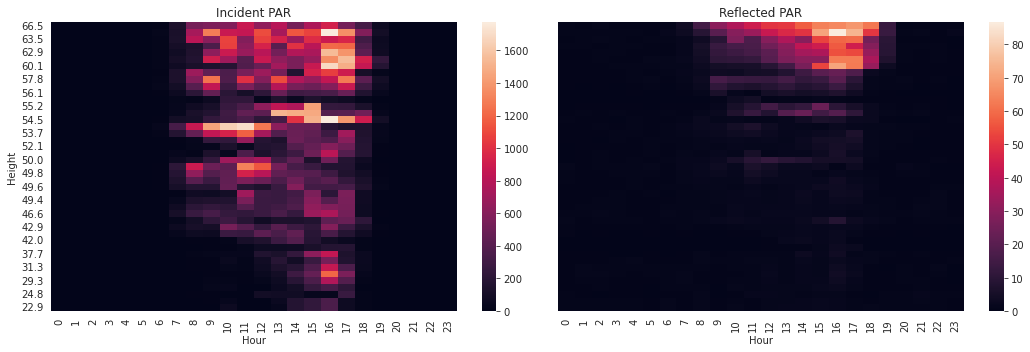
\includegraphics[width=0.7\textwidth]{eda_3.2.png}
\captionsetup{justification=centering}
\caption{PAR Intra-Day Behavior}
\label{fig:par-intra-day}
\end{figure*}
\begin{figure*}[h!]
\centering
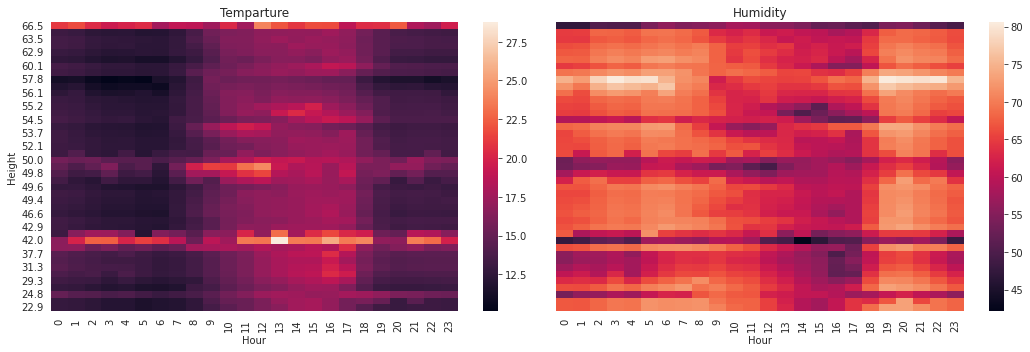
\includegraphics[width=0.7\textwidth]{eda_3.3.png}
\captionsetup{justification=centering}
\caption{Temperature and Humidity Intra-Day Behavior}
\label{fig:th-intra-day}
\end{figure*}


\paragraph{Inter-Day Temporal Trend}
Now we move away from the intra-day variations to the inter-day analysis. Here we plotted (Figure \ref{fig:ts_trend}) the first 4 days of the experiment because it has the highest data yield and quality. We can see that Temperature and Humidity vary wildly between days, and the differences in Height become less critical. On the contrary, both PAR measures follow a periodic intra-day behavior and a similar daily pattern. The differences in Height are pretty evident in Incident PAR but not that clear in Reflected PAR.
\begin{figure*}[h!]
\centering
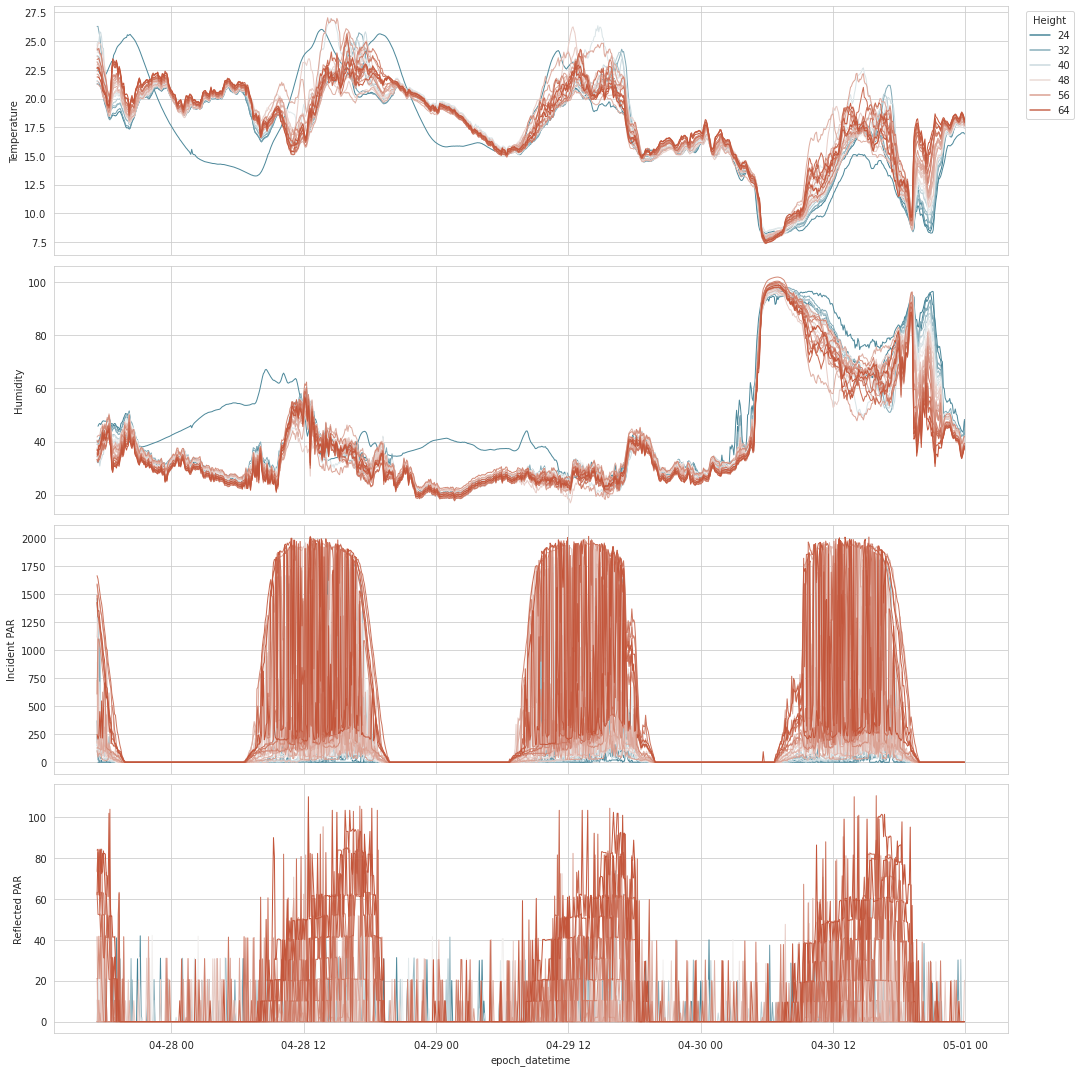
\includegraphics[width=0.7\textwidth]{eda_3.4.png}
\captionsetup{justification=centering}
\caption{4 Days Worth of Temporal Trend}
\label{fig:ts_trend}
\end{figure*}


\paragraph{PCA Analysis}
Lastly, we aggregated the data down to the sensor level. We calculated the means for all four measures (humidity, temperature, incident, and reflected PAR) at each individual hour and their metadata (height, distance, and direction). After some one-hot encoding, the result is a $\mathbf{R}^{29x105}$ matrix. We ran a PCA analysis on it and expected to see how each node behaves differently at different hours of the day concerning any of the measurements. The scree plot, Figure \ref{fig:pca_scree}, shows that the data process some lower-dimensional structures. With only 5 PC components, they explain up to 80\% of the variances. Moreover, we obtained an exciting insight by plotting the first and second PC components, Figure \ref{fig:pca_comp}, and color-coded them by each sensor's height. Most lower-level sensors experience fewer variations both during the day and the night. And those sensors located at the weather front of the tree tended to experience a significant variation in either temperature and humidity at night or larger PAR during the day.
\begin{figure*}[h!]
\centering
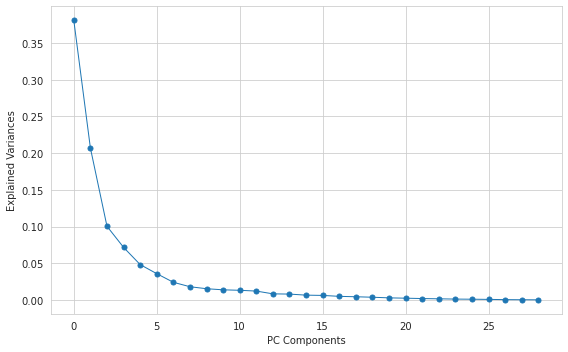
\includegraphics[width=0.4\textwidth]{eda_3.7.png}
\captionsetup{justification=centering}
\caption{PCA Scree Plot}
\label{fig:pca_scree}
\end{figure*}
\begin{figure*}[h!]
\centering
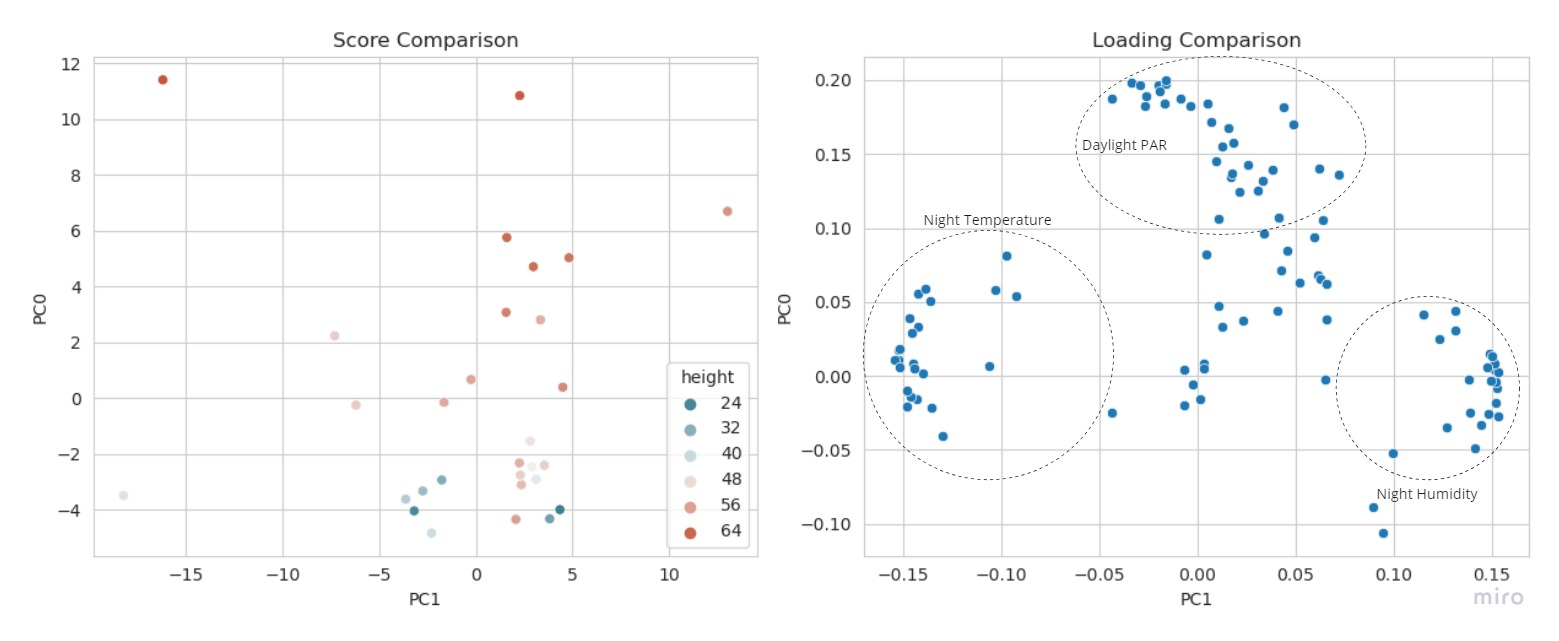
\includegraphics[width=0.85\textwidth]{eda_3.6.jpg}
\captionsetup{justification=centering}
\caption{First 2 PCA Loadings and Scores}
\label{fig:pca_comp}
\end{figure*}


\section{Interesting Findings}
\paragraph{Factor Analysis - Incident PAR with GLM}
To go further, we would like to see if we can quantify the relation between Incident PAR and other covariates. Hence, we used a Generalized Linear Model (GLM) with a Gamma sampling likelihood. Figure \ref{fig:glm_coef} shows the resulting coefficients. Despite the fact that we saw a slight relationship between PAR and Temperature and Humidity, having them in the GLM does not help with the overall RSS; hence we decided to leave them out to keep a parsimonious model. As we expected, the hour of the day holds the most influence over the Incident PAR. Next is directions. Both east and northeast tend to receive more sunlight. Height has a relatively "low" predictive power than the other covariates. It makes sense. No sensor receives radiation, no matter its height, during the night. Nevertheless, $\exp(0.0369)$ still results in $1.4\times$ more radiation per 1 meter higher than the baseline. That is a $6.3\times$ difference between the top of the tree, 70-meter, and the bottom, 20-meter.
\begin{figure*}[h!]
\centering
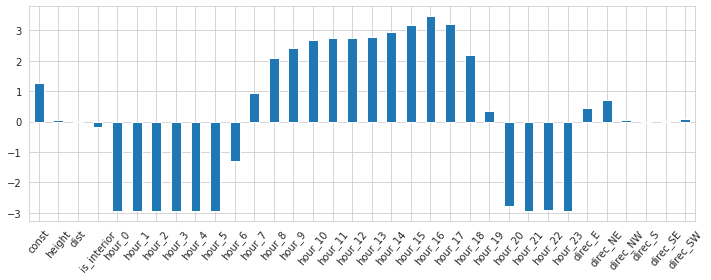
\includegraphics[width=0.7\textwidth]{eda_3.5.png}
\captionsetup{justification=centering}
\caption{Incident PAR - GLM Coefficients}
\label{fig:glm_coef}
\end{figure*}

\paragraph{Inter \& Intra Day Clustering with GMM}
Next, we used GMM to cluster inter and intra-day behaviors, assuming that the microclimate follows a low dimensional latent periodic regime change. For the inter-day relationship, we aggregated the data down to the day level, calculated the means and variances of all 4 variables, and followed a standardization treatment. The resulting GMM clusters are 3. We can see the redwood experience shift between two of the regime and occasionally switch to the third. Furthermore, for intra-day behaviors, we obtained the same features but at a 15-minute aggregation on only the date May 1st, 2004. Tolle also presented this day with a different perspective. Hence, we can have a comparison. As expected, the ideal GMM cluster for that day is 2. One for the night and one for the daytime.
\begin{figure*}[h!]
\centering
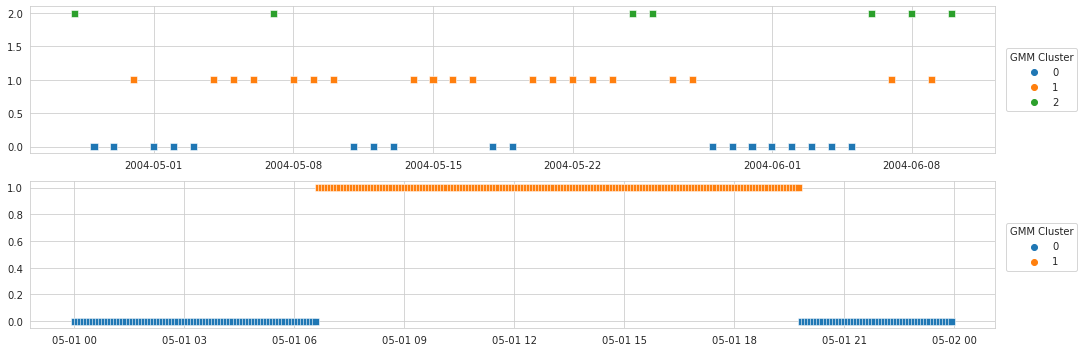
\includegraphics[width=0.8\textwidth]{if_4.3.png}
\captionsetup{justification=centering}
\caption{Incident PAR - GLM Coefficients}
\label{fig:glm_coef}
\end{figure*}

\paragraph{Inter-Day Auto-Correlation}
Even though we see that Temperature doesn't follow any obvious trend under a week, we otherwise observed a periodic behavior across the week when we started plotting the data over the entire experiment window. Figure \ref{fig:temp_autocor} shows the long-term Temperature on the left and its auto-correlation on the right. We can see that there are both large and small cycles in the Temperature variations.
\begin{figure*}[h!]
\centering
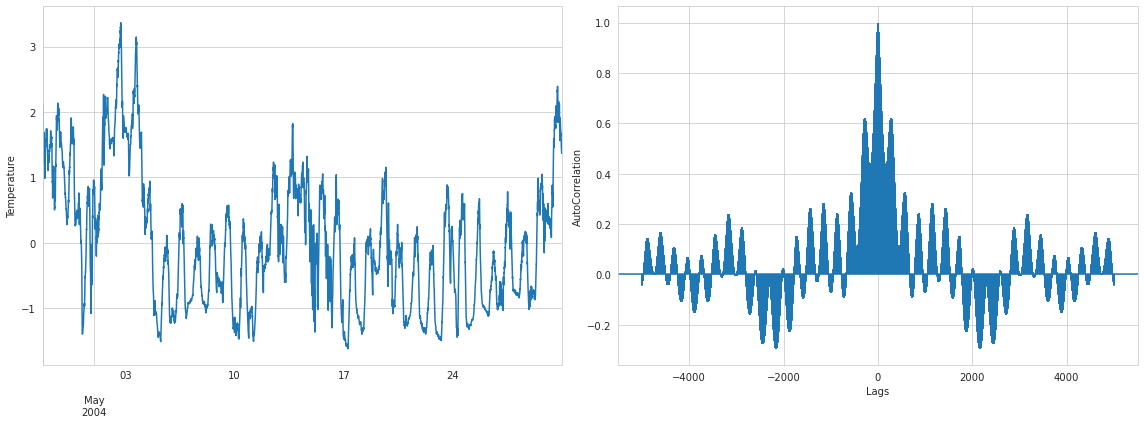
\includegraphics[width=0.8\textwidth]{if_4.4.png}
\captionsetup{justification=centering}
\caption{Long-term Temperature Auto-Correlation}
\label{fig:temp_autocor}
\end{figure*}



\section{Graph Critique}
\subsection{Part a: Log Transform of Data}
We take a log transformation on the incident and the reflected PAR and plot them. Note that since many zero values exist, we decided to split the plot into two. Firstly we plot the distribution of zero to non-zero values in a barplot; we then take a log transform of the non-zero values and plot the histogram.
\\ \\
\begin{figure}[h!]
\centering
\captionsetup{justification=centering}
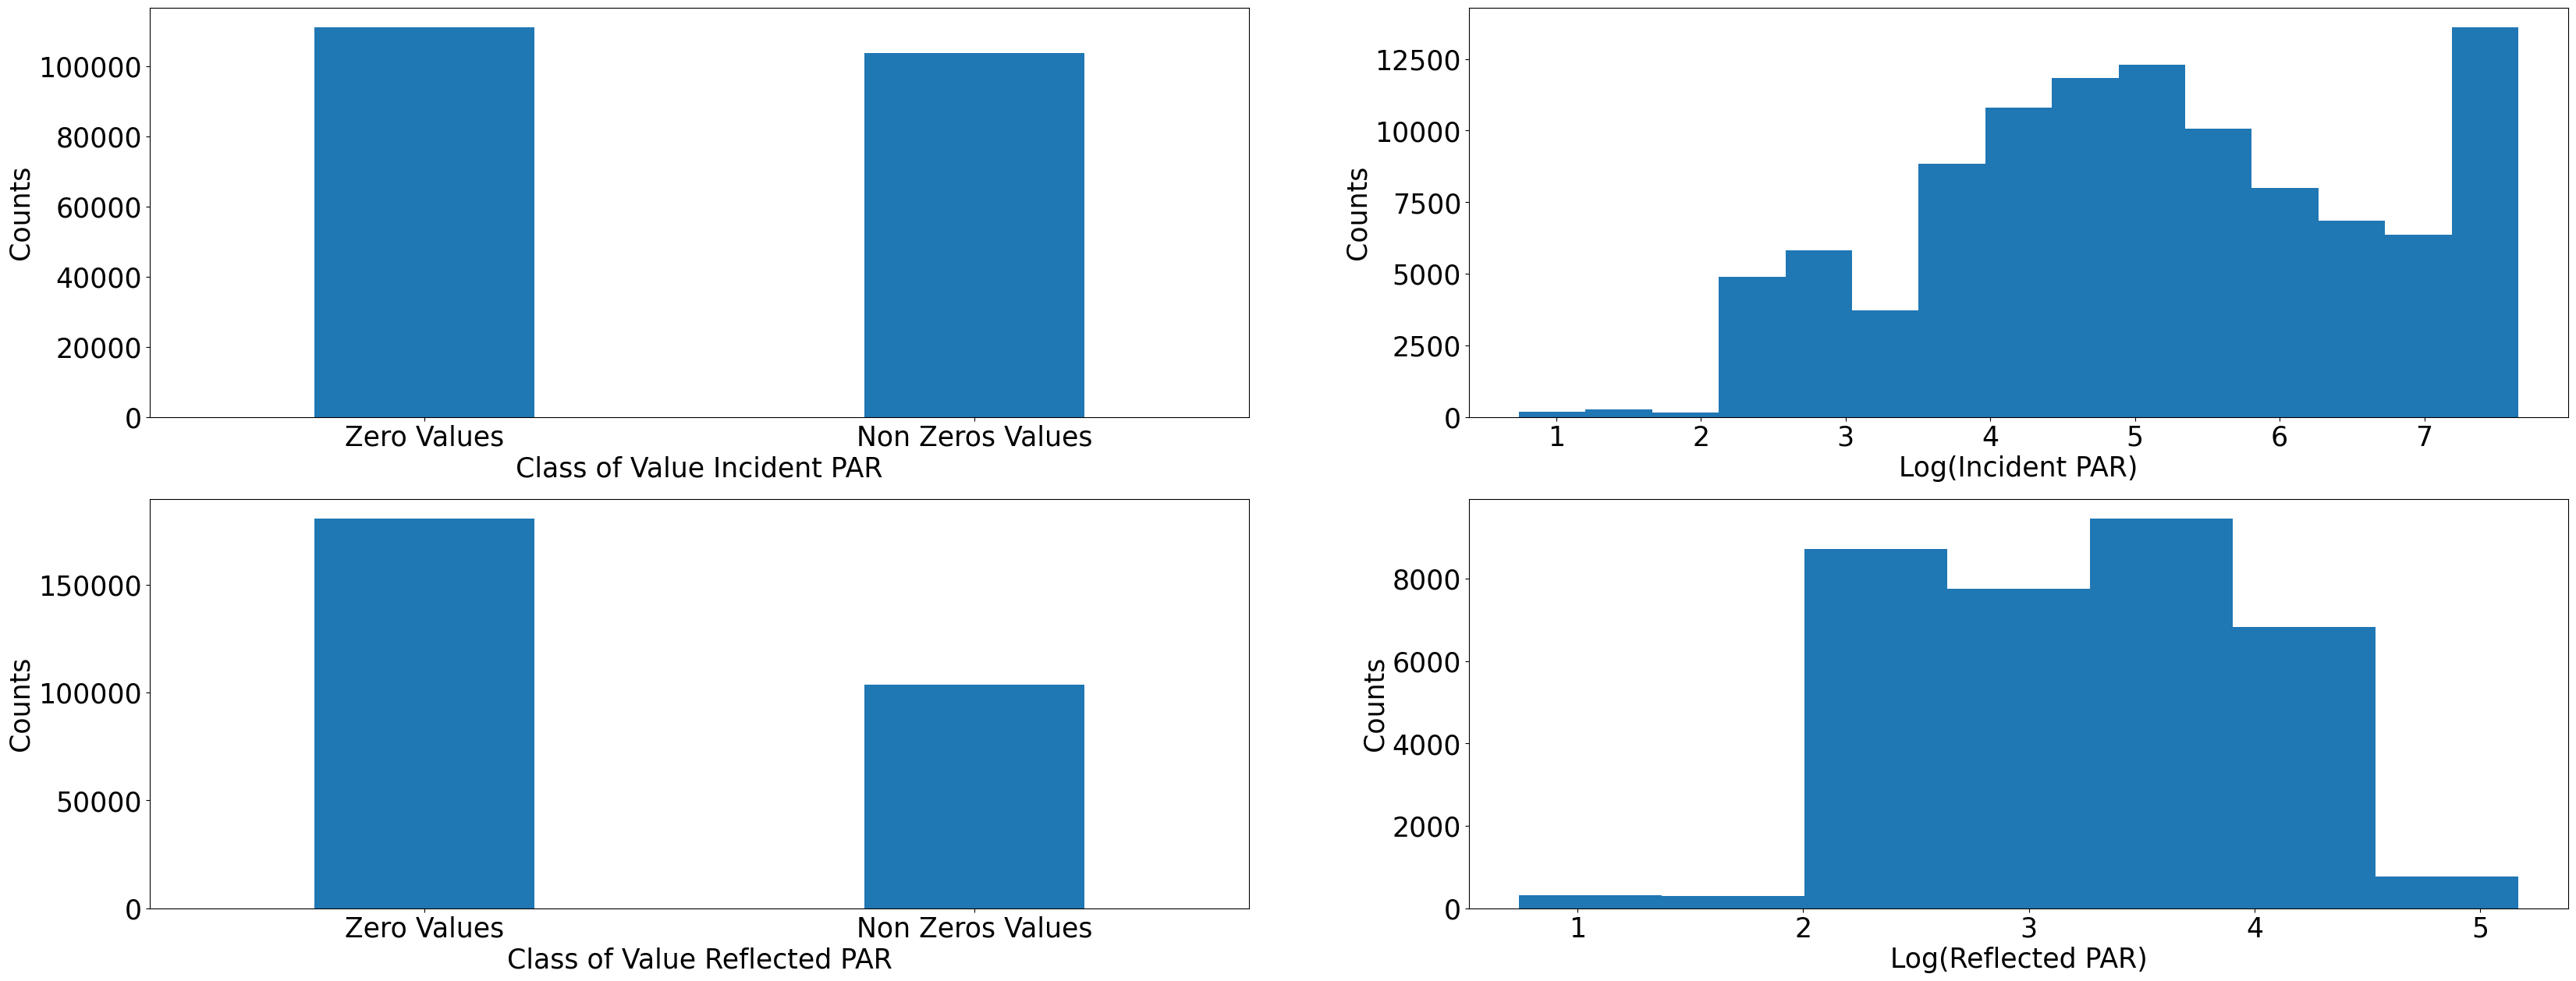
\includegraphics[width=0.9\textwidth]{Report Images/graph_critique_a_v2.png}
\caption{PAR distribution under the log transformation. Left Column: Distribution of zero vs. non-zero values. Right Column: Histogram of the log-transformed non-zero values}
\label{fig:graph_crtique_a}
\end{figure}
Figure \ref{fig:graph_crtique_a} shows the log-transformed Incident and Reflected PAR. We can see the large number of zero values. Aside from that, we see that the remaining non-zero log incident PAR values have a bimodal distribution, with a mode around 5 and close to 8. For reflected PAR, we see that majority of the data points are 0, with the remaining values ranging from 2-4; we see no discernible distribution here.

\subsection{Part b: Boxplot Evaluation}
We note two issues with the boxplots.
\begin{enumerate}
    \item We know there are significant variations in the data across time. Hence it might be misleading to summarise all the data using multiple boxplots across time.
    \item We know that the distribution for incident PAR and reflected PAR is zero-inflated and multimodal. Hence summarising in a boxplot can be misleading.
\end{enumerate}
We focus on point 2, as the author meant to remove the time dimension in the plot. Compared to Figure 4 of the paper, we see that incident PAR, and reflected PAR has many zero values at the sampled time point. This is something the boxplot representation fails to capture. \\
Instead, we have plotted a similar diagram with each boxplot replaced by a KDE plot of the log-transformed values. Note that we have added a small constant to the zero values. This is plotted in Figure \ref{fig:graph_crtique_b} for Incident PAR as an example. Note also that we have sub-sampled the heights to create a more reasonably sized plot. With the KDE, we can see clearly both a large number of zeros as well as the shifting distribution of the non-zero values as the height increases.
\begin{figure}[h!]
\centering
\captionsetup{justification=centering}
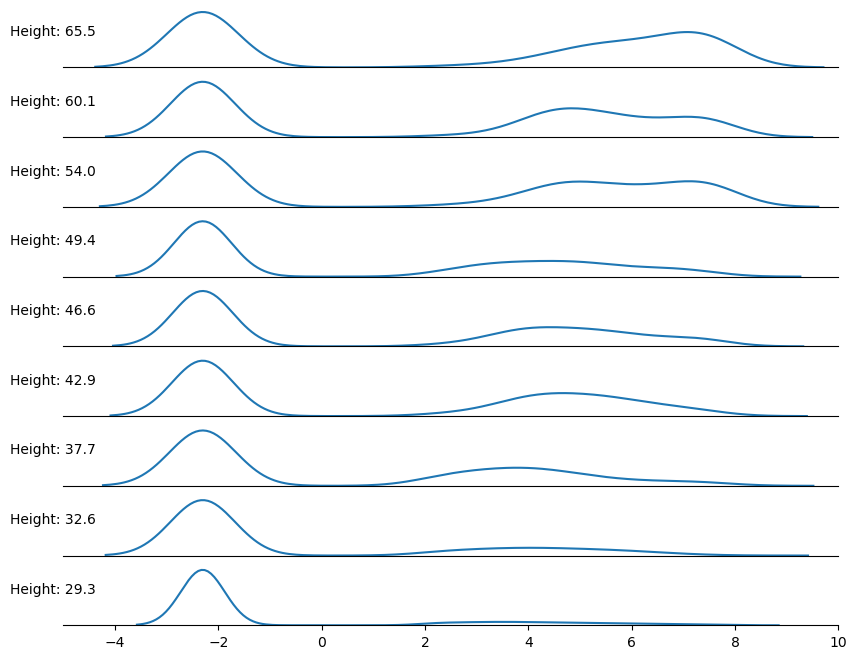
\includegraphics[width=0.8\textwidth]{Report Images/Fig7_graph_criqitue_bv2.png}
\caption{Incident PAR distribution under the log transformation}
\label{fig:graph_crtique_b}
\end{figure}
\\

\subsection{Part c: Sequence Plot Evaluation}
The authors have plotted each node's readings with a unique color. Due to the large number of nodes, the colors are hard to distinguish, and it is generally hard to pick out any trends. Instead, we consider an alternative where we color each curve by its height according to a color gradient. This is shown in Figures \ref{fig:graph_crtique_c1} and \ref{fig:graph_crtique_c2}.
\\
\\
Generally, one would use a sequential color bar to represent this information. However, we found the sequential color bars hard to see due to the large range of heights, even after normalization. Hence we chose to use a diverging color bar instead. See from Figures \ref{fig:graph_crtique_c1} and \ref{fig:graph_crtique_c2} that the plots now show us a very clear trend that higher up nodes have lower humidity and higher temperature lower height nodes have higher humidity and lower temperature.  This is new information that the previous graph of the authors was unable to showcase in the paper.
\begin{figure}[h!]
\centering
\captionsetup{justification=centering}
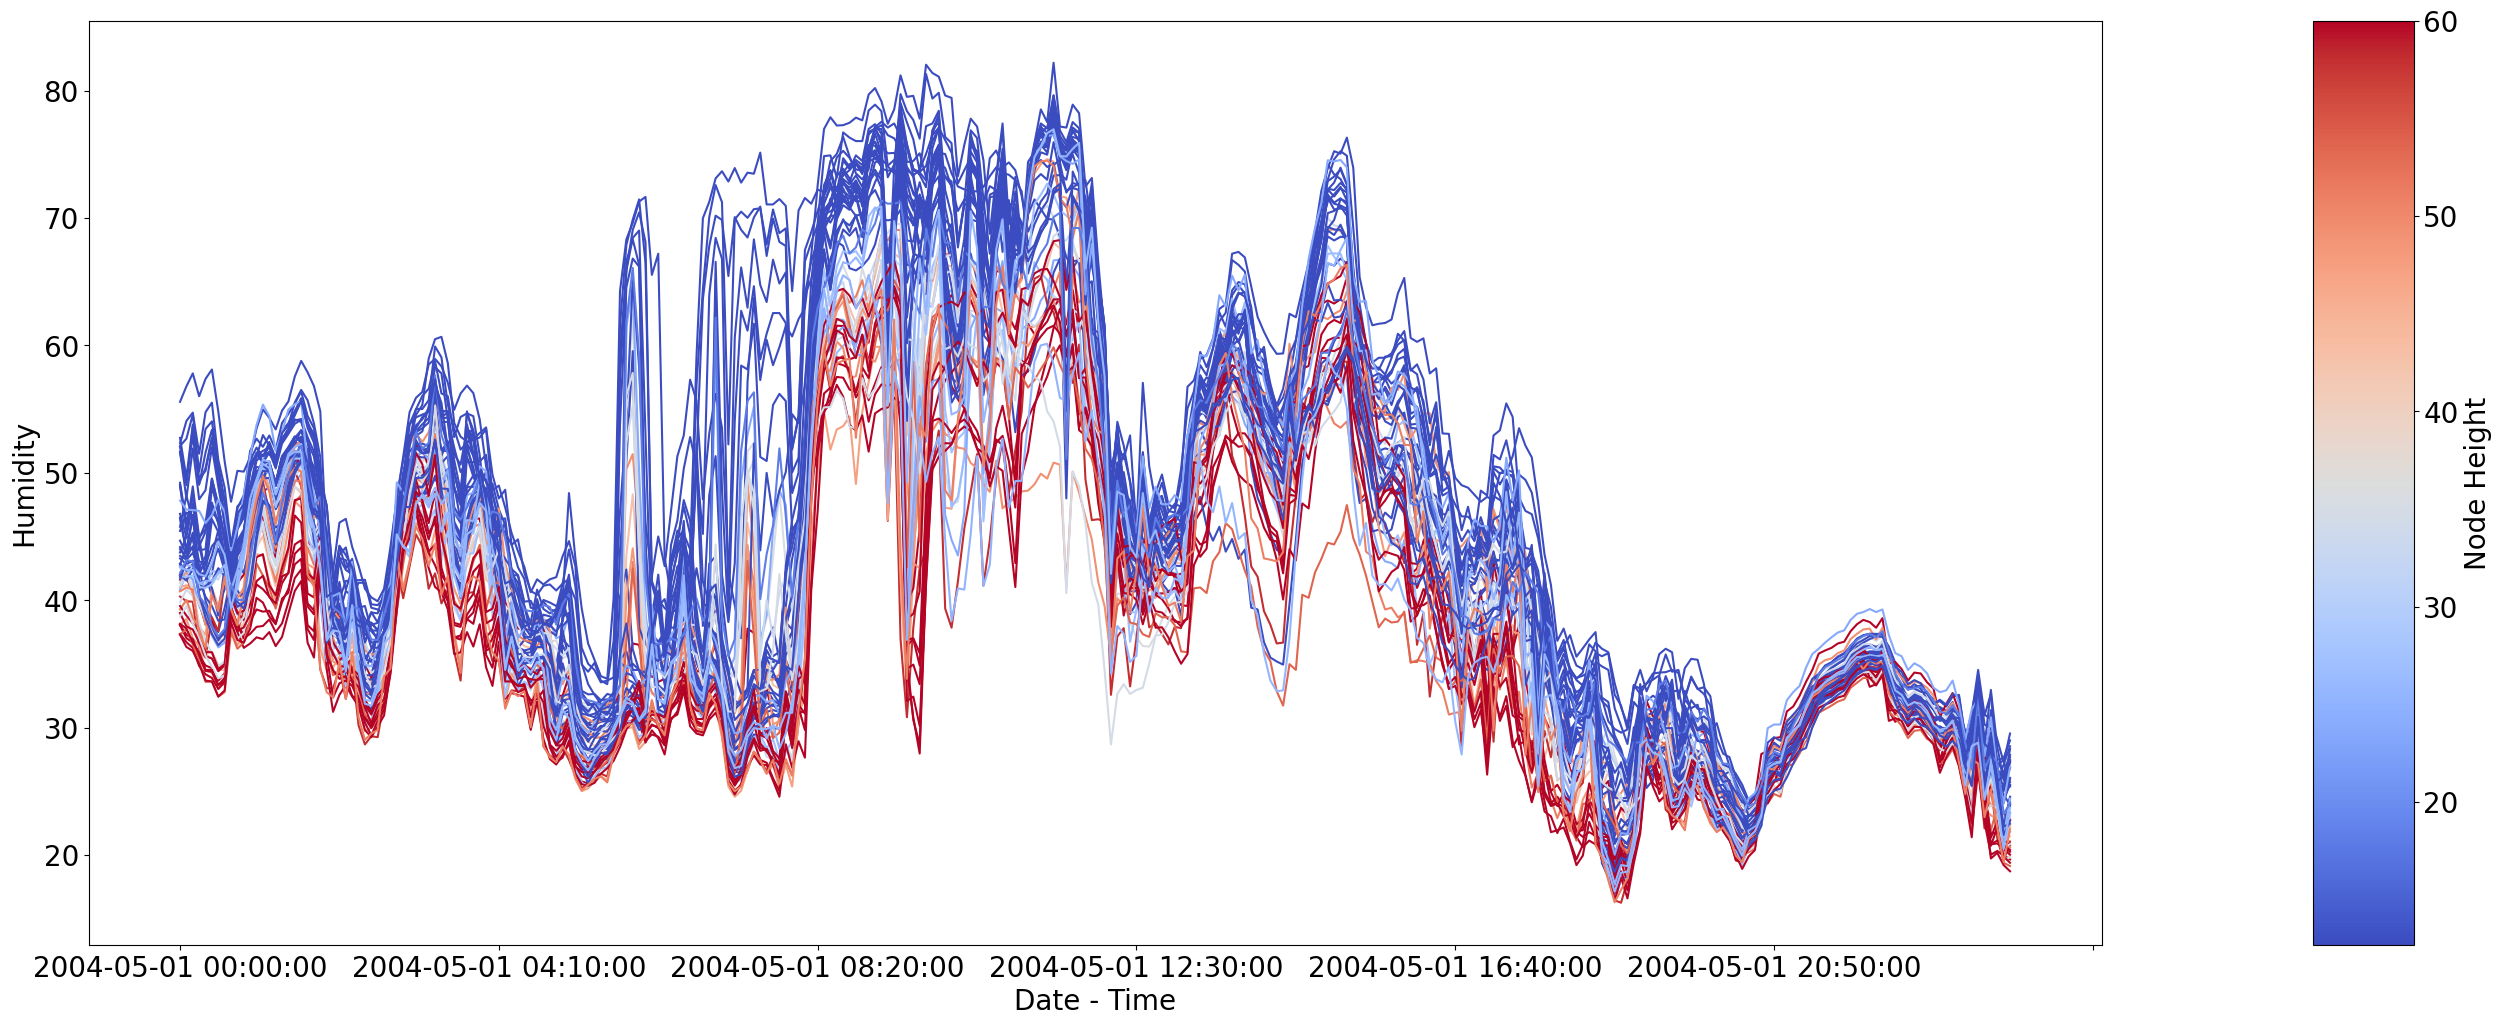
\includegraphics[width=0.8\textwidth]{Report Images/fig8_graph_critique_c1.png}
\caption{Time Series of Humidity Values Per Node with Curves Colored by Node Height}
\label{fig:graph_crtique_c1}
\end{figure}
\\
\begin{figure}[h!]
\centering
\captionsetup{justification=centering}
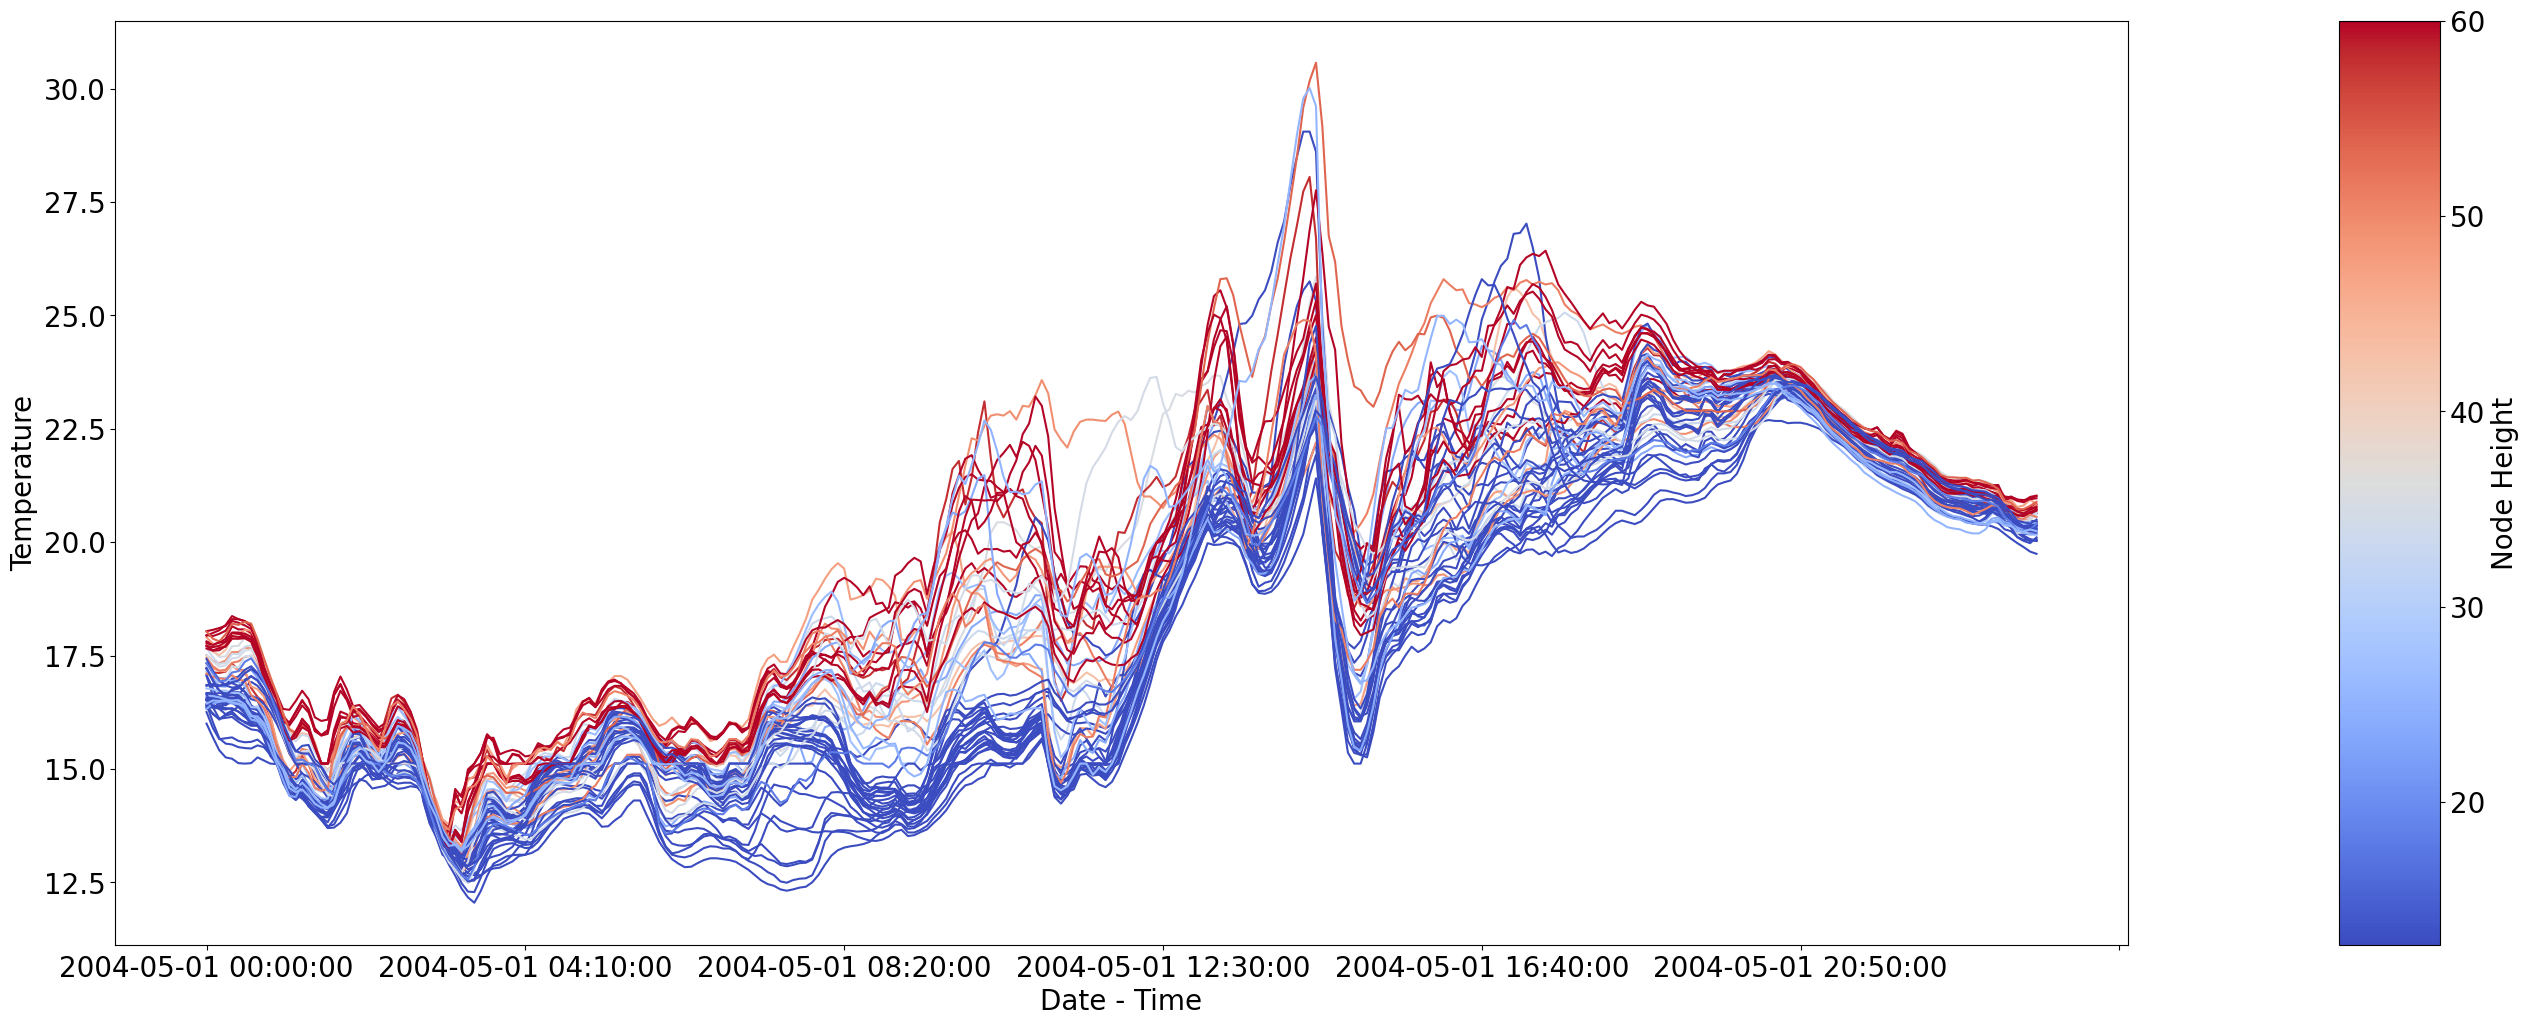
\includegraphics[width=0.8\textwidth]{Report Images/fig8_graph_critique_c2.png}
\caption{Time Series of Temperature Values Per Node with Curves Colored by Node Height}
\label{fig:graph_crtique_c2}
\end{figure}


\subsection{Part d: Differences in Network and Log}
The main issue we find with Figures 7a and 7b of the paper is that the network and log data are plotted separately. This can make comparisons between the two difficult. We also found that the leftmost plot does not convey useful information that is not already available in the other three graphs; hence we dropped it.  Lastly, we found that the second leftmost plot is messy when plotted using the boxplot. Therefore, we only plot the daily average percentage yield to underscore the differences. 
\\
\begin{figure}[h!]
\centering
\captionsetup{justification=centering}
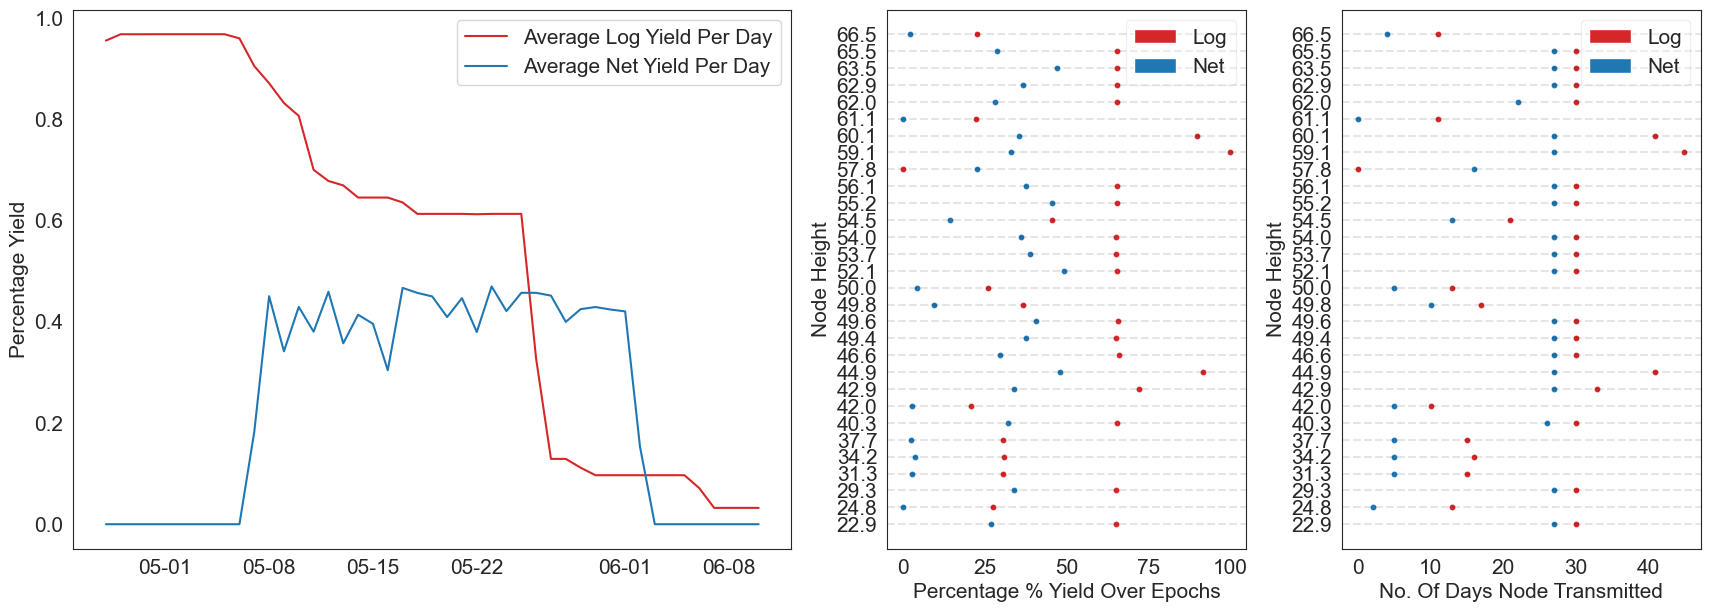
\includegraphics[width=1\textwidth]{Report Images/graph_critique_d.png}
\caption{Reworked Comparisons Between Network and Log Data Yield}
\label{fig:graph_crtique_d}
\end{figure}
\\

Figure \ref{fig:graph_crtique_d} shows our modified version of Figures 7a and 7b. As can be seen, the net and log information are plotted onto the same axis, allowing easier comparison. We can see clearly that the log yield generally exceeds the net yield for almost all nodes. Further, the log tends to be operational for more days than the network storage. 

\pagebreak

\begin{appendices}

\section{Features in Data}
% the \\ insures the section title is centered below the phrase: Appendix B

\begin{multicols}{3}
\begin{itemize}
    \item result\_time
    \item epoch
    \item nodeid
    \item parent
    \item voltage
    \item humidity
    \item humid\_temp
    \item humid\_adj
   atem Incident\_PAR(hamatop)
    \item Reflected\_PAR(hamabot)
    \item Height
    \item Direc
    \item Dist
    \item Tree
\end{itemize}
\end{multicols}

\end{appendices}

\end{document}




We saw one sensor that is consistently producing theoretically out-of-range data.

The voltage value in the logging file is different in the network dataset. Also, voltage gives out a signal on the battery life. We shall consider removing data points when the sensors are near the end of the battery life.

We have around 73 unique nodes in the logging data but only 31 on the network data.

Sometimes we can have multiple measures at the same epoch, which might also have variations within them.

Sensors have measuring error bound, so we can't mindlessly filter out the data points.


\end{document}